\subsection{特異型EEJの自動判定手法}
\label{sec:peculiar_eej_detection}

本研究では、特異型EEJを定量的に抽出し分類するために、以下の手順で自動判定を行った。
先行研究である \citeauthor{Ikesue2024}\citetype{Ikesue2024} (\citeyear{Ikesue2024}) では、目視によって特異型EEJの分類が行われていたが、定量的な評価を行うためには客観的な自動判定手法が必要である。
また、同研究では特異型EEJの発生数を用いて評価が行われていたが、観測データの欠損や地磁気擾乱による除外期間の影響を考慮すると、発生数ではなく発生率を用いて評価を行うことが望ましい。

さらに、先行研究で定義された「その他型」は、地磁気擾乱日においても類似した波形が観測されることが確認された。
そのため、本研究では「その他型」を特異型EEJの定義から除外し、地磁気静穏時に特有の現象である「未発達型」および「突発型」の2種類のみを抽出対象とする。
このとき、Dip赤道上のEEJが抑制される現象を包括的に調査するため、先行研究における「CEJ型」と「急落型」は区別せず、一括して「突発型」として定義する。

以下では、ペルー・ブラジル領域におけるMAGDAS観測点（ANC, HUA, EUS）のデータを例として、その手順を示す。
\subsubsection{指標の定義}
準静穏日（Kp < 4 かつ EDst > -30 nT）を対象とし、Dip観測点（ANC, HUA）およびOffdip観測点（EUS）のEUELの日最大値（ピーク値）の差を算出し、その分布を作成する。

\begin{equation}
 \Delta_{peak} EUEL = \text{max}(EUEL_{\text{dip}}) - \text{max}(EUEL_{\text{offdip}})
\end{equation}


\subsubsection{特異型EEJの抽出}
算出されたEUELピーク差分布の下位10\%の値を閾値として設定し、この閾値を下回るイベントを特異型EEJとして定義した。
ペルー・ブラジル領域の例では、$\Delta_{peak} EUEL < 12.8$ nT を満たす日が特異型EEJとして抽出される。

\begin{figure}[htbp]
  \centering
  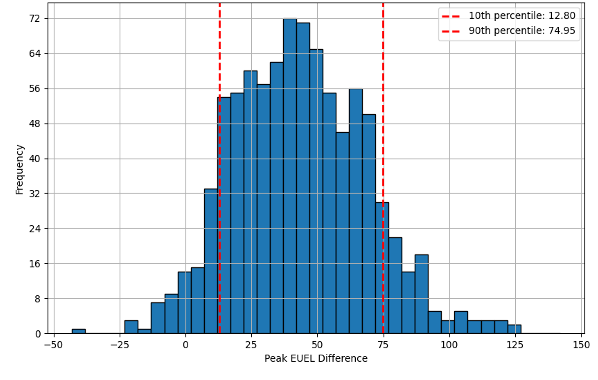
\includegraphics[width=0.8\textwidth]{figures/anc_hua_eus_euel_histgram.png}
  \caption{EUELピーク値差の分布}
  \label{fig:euel_difference_histogram}
\end{figure}


\subsubsection{特異型EEJの分類}
次に、抽出された特異型EEJイベントを未発達型および突発型に分類するため、
Dip観測点とOffdip観測点におけるEUELの時間変化の相関係数を算出した。
EUELが両観測点で類似した変動を示す場合には相関係数は高い値を示す。
一方、Dip観測点のみで急激な減少などの異なる変動が生じた場合には、相関係数は小さくなる。
この性質を利用することで、特異型EEJを二つのタイプに分類することが可能となる。
なお、朝方及び夕方にCEJの効果を強く受け、未発達型であるのにもかかわらず突発型として誤判定される可能性があるため、
本研究では、ペルー・ブラジル領域においては、昼間の時間帯（9:00 LT $\sim$ 15:00 LT）のみのEUELの波形の相関係数を算出し、
ブラジル領域においては、10:00LT $\sim$ 16:00LTのみのEUELの波形の相関係数を算出した。


\begin{itemize}
    \item \textbf{未発達型 (Undeveloped type)}：
    Dip観測点とOffdip観測点のEUEL間の相関係数が0.6以上のイベント。
    波形の時間変化が類似しており、主として振幅差のみが小さい場合に対応する。
    \item \textbf{突発型 (Sudden type)}：
    Dip観測点とOffdip観測点のEUEL間の相関係数が0.6未満のイベント。
    波形の形状自体が異なり、Dip観測点における突発的な減少などを伴う場合に対応する。
\end{itemize}

なお、本節で示した閾値（ピーク値差および相関係数）はペルー・ブラジル領域(ANC, HUA, EUS)の観測点配置に基づくものであり、
他地域に適用する場合には、観測点配置や統計的特性に応じて閾値を再設定する必要がある。